% ---------------------------------------------------%
% DISCLAIMER: ADA KEMUNGKINAN BAB 3 STRUKTUR YG DIBAHAS BERBEDA, JADI DI BAWAH ADA CONTOH
% BAB 3 KATING. MODIF SAJA SESUAI KEBUTUHAN

% ---------------------------------------------------%

% \chapter{Analisis dan Perancangan}
\chapter{Analisis dan Rencana Penelitian}

\section{Analisis Masalah}

Dalam mengimplementasikan protokol komunikasi dengan memanfaatkan cipher simetris dengan kunci dinamis dengan memanfaatkan sistem \emph{chaos}, terdapat beberapa permasalahan yang muncul. Permasalahan pertama adalah metode untuk melakukan sinkronisasi sistem \emph{chaos} dengan jumlah komunikasi yang konstan. Sistem \emph{chaos} ini digunakan sebagai \emph{state} yang dimanfaatkan untuk mengatur keteracakan pada hasil enkripsi menggunakan AES, sehingga diperlukan sistem \emph{chaos} yang tersinkronisasi. Selain itu, komunikasi memungkinkan dilakukan pada jaringan yang kurang reliabel.

Permasalahan kedua yang muncul dengan mengimplementasikan protokol ini adalah metode untuk melakukan enkripsi tanpa perlu mengubah internal dari AES standar. Saat ini, proses enkripsi memanfaatkan AES dapat dijalankan dalam level instruksi mesin seperti yang tertulis pada \textcite{gueron2010}. Pengubahan internal AES standar dapat menyebabkan instruksi AES standar tidak bisa digunakan lagi.

Permasalahan ketiga yang muncul adalah metode untuk mengirimkan pesan semetode \emph{full-duplex}. Saat ini, semetode lumrah komunikasi antar dua buah pihak dapat dilakukan semetode \emph{full-duplex}. Akan tetapi, pengiriman memanfaatkan kunci yang dinamis memerlukan kedua belah pihak menyimpan state yang sama untuk melakukan enkripsi dan dekripsi. Oleh karena itu, diperlukan sebuah metode agar proses ini dapat dilakukan semetode sinkron tanpa menghilangkan sifat \emph{full-duplex}.

Dalam komunikasi pada jaringan yang tidak aman, dimungkinkan terjadinya penerimaan data dari pihak yang tidak sah. Hal ini dapat menimbulkan permasalahan pada protokol dikarenakan dapat mengancam ketersinambungan \emph{state}. Oleh karena itu, metode untuk memastikan pesan dapat diotentikasi dan metode penanggulangan apabila proses otentikasi gagal.

\section{Analisis Solusi} 

Berdasarkan \textcite{lin2021}, proses sinkronisasi dapat dilakukan dengan metode mengirimkan parameter sinkronisasi untuk sistem chaos. Kekurangan metode ini adalah jumlah komunikasi yang diperlukan cukup banyak sehingga kurang efektif bila dilakukan pada jaringan kurang reliabel. Metode lainnya yang dapat dilakukan adalah dengan memanfaatkan algoritma pertukaran kunci Diffie-Hellman sebagaimana yang dilakukan pada protokol SSL sebagaimana yang dijelaskan pada \textcite{munir2019}.

Proses pengenkripsian pesan secara dinamis dapat dilakukan dengan memanfaatkan kunci blok. Dengan melakukan hal ini, proses enkripsi pada internal AES tidak perlu berubah. Selain itu, keteracakan kunci blok akan menjamin hasil enkripsi akan berbeda walaupun memiliki pesan yang sama sebagaimana pengujian yang dilakukan oleh \textcite{lin2021}.

Untuk mengirimkan data secara \emph{full-duplex}, dapat dilakukan dengan metode memisahkan sistem \emph{chaos} untuk melakukan pengiriman dan penerimaan data. Hal ini dapat menjamin pengiriman data dapat dilakukan secara bersamaan. Bagi pengirim, Nilai sistem \emph{chaos} akan diupdate jika proses pengiriman telah mendapatkan konfirmasi. Bagi penerima, Nilai sistem \emph{chaos} akan diupdate jika proses pengiriman telah mendapatkan blok pesan baru dari pengirim.

Dalam melakukan verifikasi pesan, dapat dilakukan sebuah metode yaitu dengan cara memanfaatkan HMAC. Setiap pesan yang diterima perlu diperiksa melalui HMAC dengan kunci blok yang digunakan pada pendeskripsian blok sebelumnya. Apabila pesan yang diterima sah, sistem \emph{chaos} akan diperbaharui. Nilai sistem \emph{chaos} selanjutnya akan digunakan untuk mendekripsi pesan tersebut.

\section{Gambaran Solusi}

Proses enkripsi dan dekripsi yang dilakukan pada protokol yang akan dibangun digambarkan pada figur \ref{fig:solution.encrypt} dan \ref{fig:solution.decrypt}. Mode blok enkripsi yang akan digunakan adalah \emph{cipher block chaining} (CBC). Setiap blok pesan yang dikirimkan akan diberikan sebuah MAC sebagai otentikasi dari pesan yang dikirimkan. Apabila dalam pengiriman blok mengalami kegagalan dikarenakan kegagalan otentikasi, pesan akan diretransmisi ulang. 

Dalam melakukan pengiriman, pembangkitan kunci baru pada sisi pengirim dilakukan saat telah melakukan enkripsi dalam suatu blok. Pada sisi penerima, pembangkitan kunci dilakukan setelah menerima blok baru. 

\begin{figure}[!h]
  \centering
  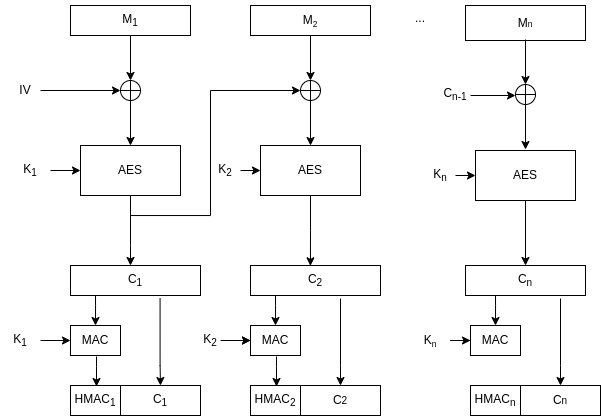
\includegraphics[width=250px]{chapters/res/chapter-3/img/encrypt.png}
  \caption{Enkripsi Pesan secara Dinamis} \label{fig:solution.encrypt}
\end{figure}

\begin{figure}[!h]
  \centering
  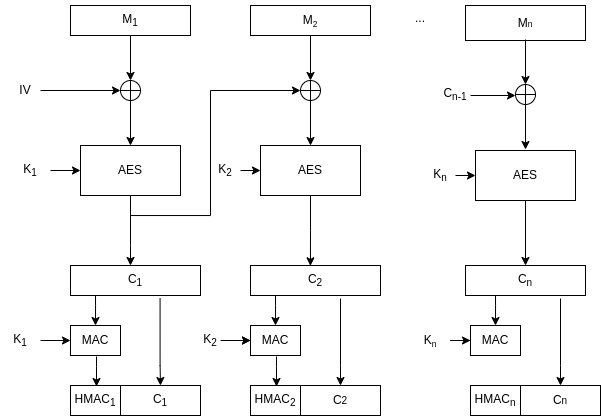
\includegraphics[width=250px]{chapters/res/chapter-3/img/encrypt.png}
  \caption{Dekripsi Pesan secara Dinamis} \label{fig:solution.decrypt}
\end{figure}
